\section{Project Control}

\subsection{Association status}

Rathaxes is an "Association loi de 1901" (a non-profit assocation). An update of
the statuses is planned for late 2010.

A bank account managed by the association will be created to sustains the needs
of the project.

Planned outgoings:
\begin{itemize}
\item Peripheral purchases (mouses, network cards, \ldots);
\item Travels (RMLL\footnote{Rencontre Mondiales du Logiciel Libre
(\url{http://rmll.info/}).}, Fosdem\footnote{\url{http://www.fosdem.org/}.});
\item Domain name (rathaxes.org).
\end{itemize}

As an association Rathaxes is able to receive donations.

\subsection{Work environment}

\begin{itemize}
\item The LSE is able to meet most of the hardware needs;
\item Three operating systems will be used for researches and tests, three x86
computers will be needed. These computers can be virtualized in order to unify
the test environment;
\item Test peripherals will be obtained from the LSE stock or purchased if
needed
\item The code is hosted by GoogleCode at:
\url{http://code.google.com/p/rathaxes/};
\item The google code wiki provides a starting point to install and test
Rathaxes;
\item The code is versionned with
Mercurial\footnote{\url{http://mercurial.selenic.com/}.};
\item The bug tracker is public and used to develop the project;
\item Code, tickets, documentation must be written in english;
\item In addition of the mailboxes provided by Epitech each member must be
present on the following IRC channel: \url{irc://rathaxes@irc.freenode.org/}.
\end{itemize}

\subsection{Planification}

Rathaxes 2012 is the sum of multiple steps:

\begin{enumerate}
\item study of existing drivers on each platform;
\item write C drivers on each platform;
\item define concepts to implement in the DSL;
\item start to work again the Rathaxes code;
\item upgrade the DSL;
\item write peripheral drivers with Rathaxes;
\item apply to the RMLL and Fosdem.
\end{enumerate}

\begin{center}

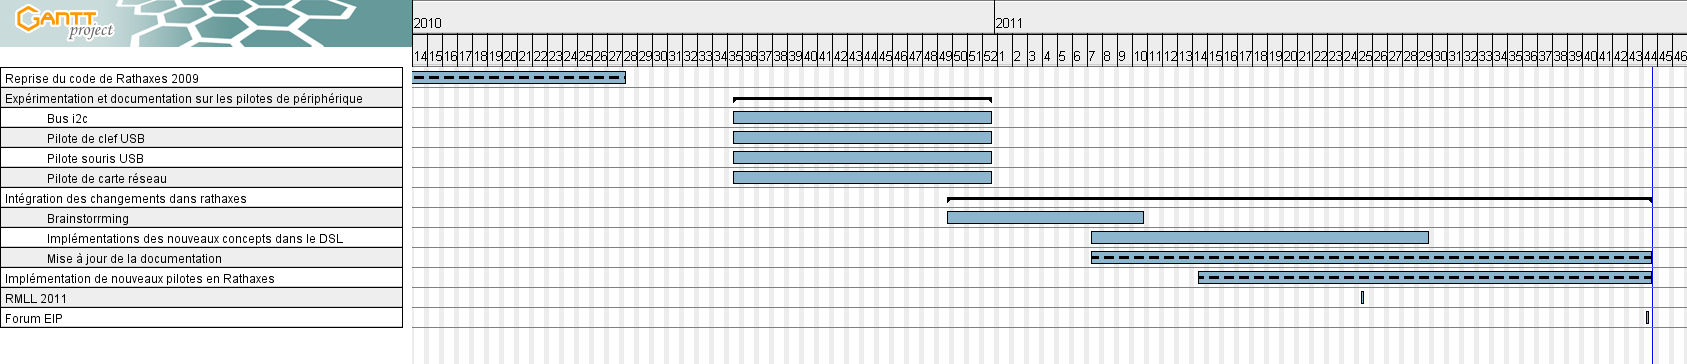
\includegraphics[angle=90,scale=0.35]{../images/gantt}

\end{center}
